\section{Probing extra galactic sources}
%In this section one will look at different observables and methods of probing extra galactic sources as potential candidates for the origin of the UHECRs and/or neutrinos. The goal is to constrain our list of candidates by applying known effects and theoretical models to observed data. In brief one will be discussing, The hillas criterion, the anisotropy of the UHECRs and neutrinoes, "the emissivity of our sources in UHECRs and neutrinos", and a comprehensive time scale analysis of the sources.

In this section one will outline some different methods and observables used to probe extra galactic sources as potential candidates for the origin of the UHECRs and/or neutrinos. The goal is to constrain our list of candidates by applying known effects and theoretical models to observed data, and to discuss the implications of these constraints. In brief, one will be discussing the energy budget of our sources, the anisotropy of the UHECRs and neutrinos, and a comprehensive time-scale analysis of the sources. In order to do so several key pieces of information is required, which will be discussed in the following sections.


\subsection{Density and anisotropy}

Due to the non-observation of any dipole moment in the distribution of extra-galactic UHECRs, and neutrinos as discussed in section \ref{sec:high_energy_particles} one can put strict limits on the density of sources. In \cite{ThePierreAugercollaboration_2013} they quote a density larger than $(0.06-5) 10^{-4} \rm{Mpc^{-3}}$ at a $95\% $ confidence level. This density although not exceedingly large would still damper the idea of singular but powerful sources. 

To calculate the density of sources in the Universe there are several methods. The most common method is to use the luminosity function of the sources in question.
The luminosity function is a function that describes the number of sources per unit volume and luminosity. Typically, the focus is on the differential luminosity function, which is defined as
\begin{equation}
    \frac{d\Psi(L,z)}{dL} = \frac{d^2N(L,V_c(z))}{dLdV_c(z)}.
\end{equation}

%The quantity of interest is now a number density which can be very useful in deriving observed flux of different objects here on earth. 
One also can change the differential of the comoving volume into a term only depending on the redshift assuming the source population is isotropic and by multiplying with the differential comoving volume element. This 
transformation goes as follows, 

\begin{equation}
    \frac{d^2N(L,V_c(z))}{dLdV_c(z)}\frac{dV_c(z)}{dz} = \frac{N(L,z)}{dLdz}.
\end{equation}


To effectively determine the LF, it's typical to divided it into two distinct components: a local term and a time evolution term.
 This approach involves taking the local luminosity function, calculated at a redshift 
$z=0$, and then scaling it with a function that accounts for the change in redshift. 
The exact form of the total LF varies based on the source object, but it generally falls into two categories derived from the method of incorporating the growth term into the local LF.
 These methods are selected based on which best represents the observed evolution.

 The two distinctions are the Pure Density Evolution (PDE) and the Pure Luminosity Evolution (PLE). 
 The PDE model modifies the local density function to reflect changes over time, 
 while the PLE model adjusts the local luminosity. The evolution is better represented by their equations and is given as 

 \begin{equation}\frac{d\Psi(L,z)}{d(L)} = 
    \begin{cases}
        \frac{d\Psi(L/e(z),z=0)}{d(L)} \quad (PLE)\\
        \frac{d\Psi(L,z=0)}{d(L)}e(z) \quad (PDE)\\
    \end{cases}
    .
\end{equation}


For some sources which lack obersvational data it can be difficult to estimate a full luminosity function. Due to the lack of observation or a big bias in the catalogue selection difference sources are not constrained enough and therefor one must rely on simpler estimates to get the order of magnitude. One such method given that the lifetime of a sources is know is via simple probability. One wished to estimate their required density to produce the observed amount of sources, or in the worst case one source given its average lifetime. This will in most cases serve as a lower limit, and give us a starting point for further analysis.  

in order to do so, one defines the probability of seeing a single source that has a lifetime $t_l $ up to a horizon $t$ as 

\begin{equation}
    p = \frac{t_l}{t}.
\end{equation}
The horizon is the redshift at which one stops finding appreaciable number of your source. The required density such that one observes $1$ source at present time can then be estimated as 

\begin{equation}
    n = \frac{1}{p V} 
\end{equation}

The calculation is crude, but very solid, and allows us to make lower limit estimates on sources where the Luminosity function is not defined. 

\subsection{SED broad band analysis}
The spectral shape of emitting galaxies and galaxy cores tell us a lot about the underlying dynamics, and with this information one can start to peel away the complex layers. The spectral energy distribution (SED) of a source is a plot of the energy emitted by the source as a function of frequency. In figure \ref{fig:AGN_SED} on can see the typical SED of an AGN in which the jet components, that is to say the synchrotron and inverse Compton components, are not dominant. The different components of the AGN are visible in the plot, and understanding how different components are created and contributing to the nearby enviroment will give us a better understanding of what observables one might expect from sources such as these. The main idea of these areas being good probes for UHECRs and Neutrinos is that the relativistic electrons are thought to be accompanied by relativistic protons. The true composition of the relevant areas are not known and still is a big question in this realm of research.

\begin{figure}
    \centering
    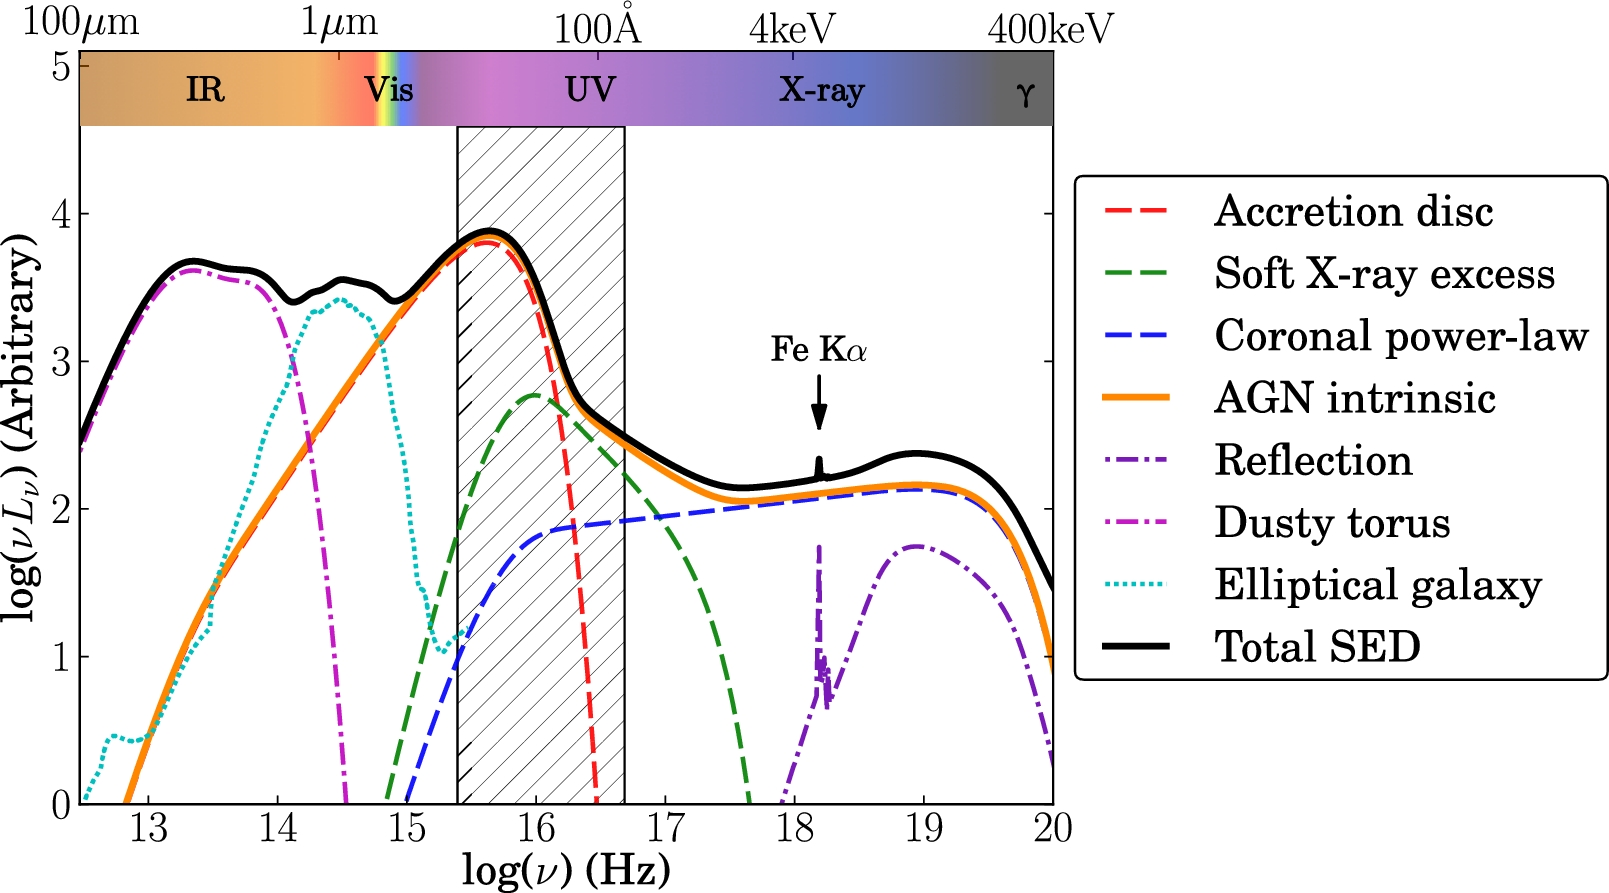
\includegraphics[width=0.7\textwidth]{C:/Users/henri/OneDrive/Documents/NTNU/Semester 10/Masteroppgave/Plots/AGN_typ_SED.jpeg}
    \caption{The spectral energy distribution of a typical AGN viewed without interference from the jet. The different components of the AGN are visible in the plot. Image taken from \cite{10.1093/mnras/stw2666}}
    \label{fig:AGN_SED}
\end{figure}

\subsubsection{X-ray energy budget}
The X-ray energy budget of especially Active galactic nuclei is often used as a probe for UHECRs and neutrino emissivity. This makes the X-ray Luminosity of AGN an interesting parameter that warrant further analysis. In this sense the X-ray luminsoity is often used a proxy for the total energy budget of escaping particles, but a true relation between the two is not known. The X-ray luminosity of an AGN usually has two sources of emission, the corona, and IC scattering of the synchrotron radiation in the jets. In both cases the main mechanism is thought to be Inverse Compton scattering and for that one requires relativistic electrons. Requiring relativistic electrons is a good indicator that there might be relativistic protons present as well, and following that logic one can start to estimate the energy budget of the protons. 


\begin{figure}
    \centering
    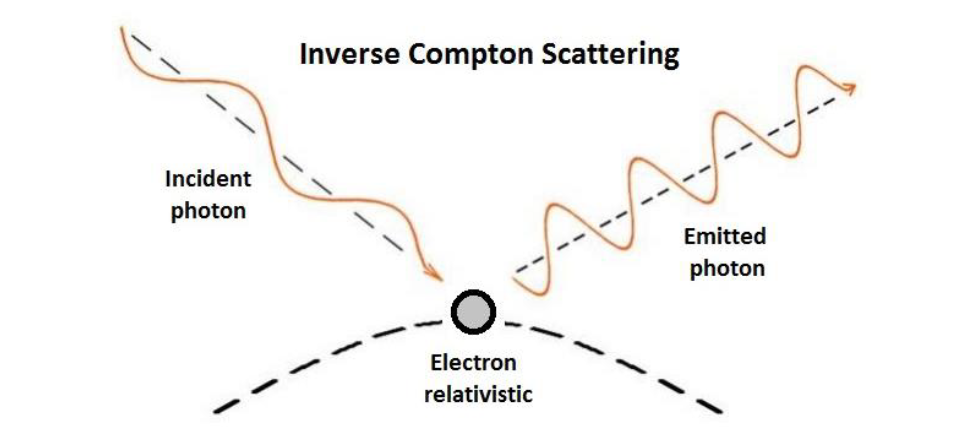
\includegraphics[width=0.7\textwidth]{C:/Users/henri/OneDrive/Documents/NTNU/Semester 10/Masteroppgave/Plots/Inverse_Compton_scattering.png}
    \caption{The inverse Compton scattering process. The process is the scattering of a low energy photon by a relativistic electron. The scattered photon will have a higher energy than the original photon. Image taken from \cite{BennumAlfred}}
\end{figure}
\subsubsection{Radio luminosity}
\subsubsection{Photon fields around AGN}
\label{sec:photon_fields}

In order to determine the photon fields we follow \cite{Ghisellini_2009} which describe the photon fields surrounding a Blazar. The photon fields separates into different contribution from the different regions of a classic AGN as discussed in section ... 
The different regions are the accretion disk, the broad line region, the torus and the x-ray corona. 


\textbf{Accretion disk:} The photon field emerging from an accretion disk if calculated by assuming a black body spectrum at each ring of an Shakura-Sunyaev disk and summing up its contributions. The temperature of 
each ring in the disk is given by 

\begin{equation}
    T(R) = \left(\frac{3 R_{S} L_{d}}{16 \pi R^3 \eta \sigma_{\mathrm{SB}}} \left(1-\left(\frac{3 R_{S}}{R}\right)^{\frac{1}{2}}\right) \right)^{\frac{1}{4}}
\end{equation}

Each ring of the accretion disk is assumed to be at the same temperature and emitting as a black-body spectrum. By using this temperature one can use the black body spectrum of an object with temperature T to find the intensity:

\begin{equation}
    \label{eq:BB}
    I(\nu) = \frac{2 h \nu^3}{c^2} \left(\frac{1}{\exp\left(\frac{h \nu}{k_B T}\right) - 1}\right)
\end{equation}

By integrating the intesity over all annuli of the disk one can find the total flux of the disk and from there the total energy density of the disk per frequency.
This then needs to be scaled to incorporate the location of our emitting region which sits at a distance $R$ from the accretion disk. 

The resulting spectral energy density is then given by

\begin{equation}
    U_d(\nu) = \frac{2\pi}{c} \int_{\mu_d}^1 I(\nu) d\mu
\end{equation}
where $\mu_d$ is the cosine of the angle between the location on the disk and the normal of the disk with respect to and observer.



\textbf{X-ray corona:} The photon field from the x-ray corona is assumed to be a power law spectrum with a cut off at high energies. Its total energy emitted is related to the disk Luminosity 
by the equation $L_{cor} = f L_d$ where $f$ is the fraction of the disk luminosity that is emitted by the corona. The spectral energy density of the corona is then given by 

\begin{equation}
    U_{cor}(\nu) = D(R)\left(\frac{\nu}{\nu_0}\right)^{-\alpha} \exp\left(-\frac{\nu}{\nu_{cut}}\right)
\end{equation}

The factor $D(R)$ is a scaling factor that incorporates the position of the observer in similar fashion to the disk. The integral of the spectral energy density over all frequencies should equate to the total energy density in x-ray at the location of the emitting region.

The energy density of x-ray around the central engine is given by a 

\begin{equation}
    \text{UX}(R) = \frac{f_{X} L_{d} \Gamma^2}{\pi (R_{X})^2 c} \left(1 - \mu_{X} - \beta(1 - \mu_{X}^2) + \frac{\beta^2 (1 - \mu_{X}^3)}{3}\right)
\end{equation}
where
\[
\mu_{X} = \left(1 + \frac{R_{X}^2}{R^2}\right)^{-0.5}.
\]

Here $f_{X}$ is the fraction of the disk luminosity that is emitted by the x-ray corona, $L_{d}$ is the disk luminosity, $\Gamma$ is the lorentz factor of the jet, $R_{X}$ is the size of the x-ray corona, $c$ is the speed of light, $\beta$ is the velocity of the observer in units of the speed of light.
In short the x-ray energy density stays constant until the observer is further away where it will decrease as $1/R^2$ which is to be expected.



\textbf{Broad line region:} The broad band field is assumed to be emitting a black body spectrum as in \ref*{eq:BB} which peaks at the Lyman-alpha line. The Lyman-alpha line is a spectral line of hydrogen  when the atomic electron transitions from the $n=2$ to the $n=1$ orbital corresponding to a frequency of $\nu_{\alpha} = 2.47 \times 10^{15}$ Hz. 
Similarly to the x-ray corona the spectral energy density is scaled to the region of interest and the total energy density is given by: 


\begin{equation}
    \label{eq:UBLR}
    \text{UBLR}(R) = 
    \begin{cases}
    \frac{f_{\text{BLR}} L_{d} \Gamma^2}{\pi R_{\text{BLR}}^2 c} & \text{if } R \leq R_{\text{BLR}}, \\
    \frac{f_{\text{BLR}} L_{d} \Gamma^2}{\pi R_{\text{BLR}}^2 c \beta 3} \left[2 (1 - \beta \mu_{\text{IR1}})^3 - (1 - \beta \mu_{\text{IR2}})^3 - (1 - \beta)^3\right] & \text{if } R \geq 3R_{\text{BLR}}, \\
    a R^b & \text{otherwise},
    \end{cases}  
\end{equation}
where 
\begin{align*}
    \mu_{\text{IR1}} &= \left(1 + \frac{R_{\text{BLR}}^2}{R^2}\right)^{-0.5}, \\
    \mu_{\text{IR2}} &= \left(1 - \frac{R_{\text{BLR}}^2}{R^2}\right)^{-0.5}, \\
    %b &= \log\left(\frac{\text{UBLR}(3R_{\text{BLR}}, R_{\text{BLR}}, f_{\text{BLR}}, L_{d}, \Gamma)}{\text{UBLR}(R_{\text{BLR}}, R_{\text{BLR}}, f_{\text{BLR}}, L_{d}, \Gamma)}\right) / \log(3), \\
    %a &= \frac{\text{UBLR}(R_{\text{BLR}}, R_{\text{BLR}}, f_{\text{BLR}}, L_{d}, \Gamma)}{R_{\text{BLR}}^b}.
\end{align*}


\textbf{Torus:} There is also assumed to be a dusty torus around the AGN emitting in infrared. The spectral energy density of the torus is also given by 
a black body spectrum with the temperature of the tours being set at $T_{\text{IR}} = 370$ K. The total energy density of the torus has the same relations 
as equation \ref{eq:UBLR} but with the relevant parameters for the torus.

\begin{equation}
    \text{UIR}(R) = 
    \begin{cases}
    \frac{f_{\text{IR}}L_d  \Gamma^2}{R_{\text{IR}}^2 c} & \text{if } R \leq R_{\text{IR}}, \\
    \end{cases}
\end{equation}

For illustrative purposes one can see the total spectral energy density in figure \ref{fig:photon_fields}. 


\subsection{Magnetic field constraints}

\subsubsection{Equipartition}
The most well know estimate for magnetic field strength in astrophysical sources is throught the equipartition argument. The fact that one observes synchrotron radiation implies that a source of relativistic electrons which have an energy density $U_e$ and that these electrons are in a magnetic field with an energy density $U_B$. The question that one aims to answer with the equipartition argument is what is the minimum total energy in both relativistic particles and magnetic fields required to produce the observed synchrotron radiation of a given frequency. The toal energy in relativistic particles and magnetic fields of a volume $V$ is given as 

\begin{equation}
    U_{tot} = U_e + U_B = V(u_p + u_{mag})
\end{equation}

Here $u_p$ is the energy density of all relativisitc particle, i.e. electrons, protons and heavyer ions ($Z>1$). Ions emit very little synchrotron radiation for a given energy $E$ compared to electrons, so little is know about their energy density, therefore it is common to assume 

\begin{equation}
    u_p = \eta u_e
\end{equation}

where $\eta$ is a constant $>1$and $u_e$ is the energy density of the relativistic electrons. In order to estimate the energy density of the electrons one assumse their distribuition as a powerlaw $n(E) \propto E^{-\delta}$, and their energy density becomes

\begin{equation}
    u_e = K \int_{E_{min}}^{E_{max}} E^{1-\delta} dE
\end{equation}

In order to move one it is require to know the spectrum of synchrtron radiation for one electron in a particular magnetic field. The derivation is a tedious process, and one will give the results obtained in \cite{2013Wilson} chapter 10.10 and 10.8. The radiated power of an electron peaks strongly around the critical frequency $\nu_c$ and one can then write a relation between a frequency $\nu$  and energy $E$ as 

\begin{equation}
    \nu = \frac{3}{2}\frac{eB}{m_e^3 c^5}E^2.
\end{equation}

This allows for the particle energy density to be written as 

\begin{equation}
    \label{eq:energy_density_particles}
    u_p = K \frac{\eta}{1-2n} \left(\frac{e}{m^3c^5}\right)^{n-1/2}\left(\nu_{max}^{1/2-n}-\nu_{min}^{1/2-n}\right) B^{n-1/2} = K G B^{n-1/2}
\end{equation}
by introducing the constant $n = \frac{1}{2}(\delta -1 )$. 

The energy density of the magnetic field is given as 

\begin{equation}
    u_{mag} = \frac{B^2}{8\pi}
\end{equation}

To move further one wished to eliminate the factor $K$ from our equations, and relate it to observed properties. \cite{2013Wilson} gives the emissivity of a synchrotron source for tangled magnetic fields as 

\begin{equation}
    \epsilon(\nu)  = b(n)K \frac{e^3}{m c^2}\left[\frac{3 e}{4 \pi m^3 c^5}\right]^{n} B^{n+1} \nu^{-n} = H K B^{n+1} \nu^{-n},
\end{equation}

where $b(n)$ is a function of the spectral index $n$. The observed flux density of a source with volume $V$  and at distance $R$ is given as 

\begin{equation}
    \label{eq:flux_density_eq}
    S(\nu) = \frac{V}{R^2} \epsilon(\nu) \propto B^{n+1} \nu^{-n}
\end{equation}

Using this relation one can then write the total energy density while inserting \ref{eq:flux_density_eq} as $K$ in \ref{eq:energy_density_particles} as

\begin{equation}
    U_{tot} = \frac{G}{H}R^2(S_v\nu^n)B^{-3/2} + \frac{V B^2}{8\pi}
\end{equation}

Given that one has measurments on distance, volume, flux density one can then estimate the magnetic field strength. One then argues that $U_{tot}$ should have a minimum value and one then finds the magnetic field to be 

\begin{equation}
    B_{eq} = \left(\frac{6\pi G}{H}\frac{R^2}{V}S_\nu \nu^n\right)^{2/7}
\end{equation}
This relationship between $U_B$ and $U_e$  at this minimum is very near the equipartition value, which is why this method is often called as such.

\subsubsection{Self synchrotron absorption}


The theory of synchrotron self absorption is a tool used previously for estimating magnetic field strength in spherically symmetric synchrotron sources. Synchrotron radiation is the product of charged particles traveling in a magnetic field. The radiation is emitted when the particles are accelerated which happens when an electron is spiraling in an uniform magnetic field. The light is usually highly polarized and is dependent on the electron energy and the magnetic field strength. Moving further along, synchrotron self absorption is the process where the synchrotron radiation is absorbed by the same electrons that produced it, and the effect of this is that any given volume of emitting plasma that radiate synchrotron radiation will have a frequency below which the radiation is absorbed. This frequency is called the turnover frequency, and one aims to show how one can estimate the magnetic field strength in the emitting plasma based on this information. The concept was first introduced by \cite{1983ApJ...264..296M}, but this section relies heaviliy on \cite{Hirotani_2005} for the derivation. 

Before we begin the derivation it is fitting to understand the spectrum of synchrotron radiation from a plasma. The spectrum is characterized by the peak frequency, also called the turnover frequency $\nu_m$, the peak flux density $S_m$, and naturally the spectral index $\alpha$. One referse the reader to image \ref{fig:synchrotron_spectrum} for a simple view of the synchrotron speaktrum in question. 

\begin{figure}
    \centering
    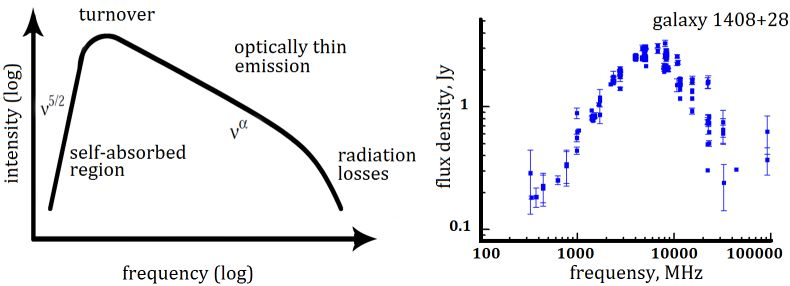
\includegraphics[width=1\textwidth]{C:/Users/henri/OneDrive/Documents/NTNU/Semester 10/Masteroppgave/Plots/SYN_spec.jpg}
    \caption{The synchrotron spectrum of a Giga hertz peaked galaxy. Later on one will realise that GHP galaxies and CSO occupy that same niche. Image taken from  Group of Active Galactic Nuclei investigation at https://www.sao.ru/hq/giag/gps-en.html }
    \label{fig:synchrotron_spectrum}
\end{figure}

In order to estimate the magnetic field strenght we must assume that it is uniform and that the electron density is also uniform. From here the transfer equation for synchrotron radiation gives in \cite{Hirotani_2005} gthe specific intensity as 

\begin{equation}
    I_\nu = A(\alpha) \nu^{*\frac{5}{2}}[1-exp(-\alpha_\nu^*x_0^* )] 
\end{equation}
where 

\begin{equation}
    A(\alpha) = \frac{3}{2}^{-\alpha}\frac{e}{c}\frac{a(\alpha)}{C(\alpha)}\left(\frac{e}{2\pi m_e c}\right)^{-3/2}B^{-1/2}
\end{equation}

and $x_0^*$ give the thickness of the emitting plasma along the observers line of sight. The coefficients $a(\alpha)$ and $C(\alpha)$ are tabulated values that depend on the spectral index $\alpha$ not to be confused with the absorption coefficient $\alpha_\nu$  and any value denoted with an asterix is in the comoving frame. 

Imagining an observer at a distance $D$ with angle $\theta$ from the blob of plasma(as seen in figure \ref{fig:Radiative_transfer}), one can define the fractional thickness, which is a Lorentz-invariant quantity, as

\begin{equation}
    \frac{x_0^*}{2R^*} = cos(\theta + \xi) = \sqrt{1-\left[\frac{sin(\theta)}{sin(\theta_d/2)}\right]^2}
\end{equation}

Determining that $\tau(0) \equiv = \alpha^*2R^*$ is the optical depth for $\theta = 0$ one can then get the full specific intensity as

\begin{equation}
    I_\nu(\theta) = \left( \frac{\delta}{1+z}\right)A(\alpha)\nu^{\frac{5}{2}}\left(1-exp \left(-\tau(0)\sqrt{1-\left[\frac{sin(\theta)}{sin(\theta_d/2)}\right]^2}\right)\right)
\end{equation}

The shape of the blob is assumed to be spherical and we can now integrate the specific intensity over the entire blob to get the total flux density as


\begin{equation}
    \label{eq:flux_density}
    S_\nu = 2\pi \int_0^{\theta_d/2} I_v(\theta)cos(\theta)\sin(\theta) = \pi sin^2(\frac{\theta_d}{2})(\frac{\delta}{1+z})^{1/2}A \nu^{5/2} \int_0^1[1-exp(-\tau(0)\sqrt{1-x^2})]dx
\end{equation}
where $x \equiv \left[\frac{sin(\theta)}{sin(\theta_d/2)}\right]^2$.
Here we insert what we know about the synchrotron spectrum and the turnover frequence $\nu_m$. We derivate the flux density with respect to frequency and set it equal to zero to find the equation that realtes $\tau_\nu(0)$ and $\alpha$ at the turnover frequency. In order to do this one needs to know the relation between the the absorption coefficient and frequency. This is given also in \cite{Hirotani_2005} as 
\begin{equation}
    \alpha_\nu^* = C(\alpha) r_0^2 k_e^*\frac{\nu_0}{\nu^*}(\frac{\nu_B}{\nu^*})^{(-2\alpha +3)/3}
\end{equation} 

where, $\nu_0 \equiv c/r_0$is the electron frequency, $r_0 \equiv e^2/(m_e c^2)$ and  
$\nu_B \equiv eB/(2\pi m_e c)$ is the cyclotron frequency. 

Having the solution for $\tau_\nu(0)$ as a function of $\alpha$ one denotes the solution at the turnover frequency as $\tau_m(0)$. This is a tabulated value and the table from \cite{Hirotani_2005} is found in the appendix.

Using this solution one can inversly solve equation \ref{eq:flux_density} for the magnetic field strength $B$ and obtain with the small angle approximation 

\begin{equation}
    B =   10^{-5} b(\alpha) \left(\frac{S_m}{\text{Jy}}\right)^{-2}\left(\frac{\nu_m}{\text{GHz}}\right)^{5}\left(\frac{\theta_d}{mas}\right)^{4}\left(\frac{\delta}{1+z}\right) \text{G}
\end{equation}

where $b(\alpha)$ is a tabulated value as well but arrises from 

\begin{equation}
    b(\alpha) = 3.98 \times 10^{3} \left(\frac{3}{2}\right)^{-2\alpha} \left[\frac{a(\alpha)}{C(\alpha)}\right]^{2} \left[\int_0^1[1-exp(-\tau(0)\sqrt{1-x^2})]dx\right]^2
\end{equation}


\begin{figure}
    \centering
    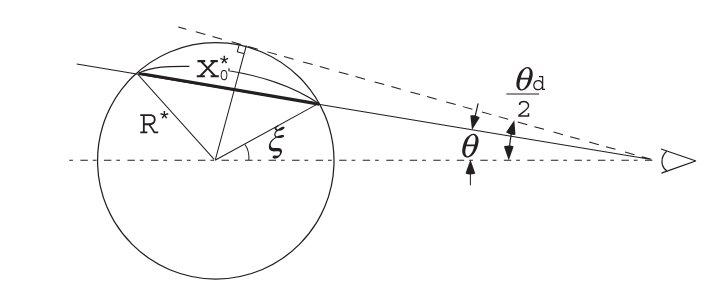
\includegraphics[width=0.7\textwidth]{C:/Users/henri/OneDrive/Documents/NTNU/Semester 10/Masteroppgave/Plots/Radiative_Transfer.png}
    \caption{Schematic view of the radiative transfer in a spherical ball of plasma. Image taken from \cite{Hirotani_2005}}
    \label{fig:Radiative_transfer}
\end{figure}

\subsubsection{Deviation from SSA and Equipartition}
If one calculates the magnetic field using both SSA and Equipartition one expects to not get the exact same results, but given a big discrepancy one cannot assume all the fault lies in only the measurments. In \cite{10.1093/mnras/stt2217} who used SSA and equipartition calculations for a small sample of CSOs, they also found a discrepancy between the two methods. The SSA had a significantly higher value for the magnetic field. This they argue can, and the weight is on can here be induced by a free free absorption effect in the source. Free free absorption is the absorption of radiation by an electron who is in close proximity to an ion. The absorption is a result of the electron being accelerated by the ion and the radiation emitted by the electron is absorbed by the ion. The effect of free-free absorption would shift the spectral peak in SSA to higher frequency and thus give a higher magnetic field strength in our calculations. This would be a good indicator that the source is harbouring ions, which one needs for UHECRs acceleration. 

\subsection{Time-scales analysis}

In order to probe what type of sources could be responsible for the observed UHECRs and neutrinos one can use the relevant time-scales a measure. The timescales of a source will act as an indicator of the dominant processes in the source, and give us an upper boundary for what we could expect of escaping particles. The dominante timescales of a source will be source specific, so further on we will be looking at the timescales of a typical compact AGN. The relevent timescales then are the acceleration timescale, the synchrotron cooling timescale, the dynamical timescale, and the photo-pion cooling timescale. 

One starts by determining the acceleration timescale of a proton undergoing first order fermi acceleration, the acceleraiton mechanisms explained in section ... . The acceleration timescale is given by the equation
\begin{equation}
    t_{acc} =  \frac{\eta \epsilon}{Z e B c}
\end{equation}
Where $\eta$ is the efficiency of the acceleration process with the most efficient acceleration harbouring the value $\eta \approx (1-10)$, $\epsilon$ is the energy of the particle, $Z$ is the charge of the particle, $e$ is the elementary charge, $B$ is the magnetic field strength and $c$ is the speed of light. 
Usually the value of $\eta$ is taken to be 1, which is the most efficient acceleration process.

The dynamical timescale is a limit on the sources size and can be estimated several ways. The sources size is important since in order to accelerate particles the source must also be able to contain particles. If one does not have good measurments on the source size, but have good fluence measurments of an attributing light curve one can estimate the size of the source via the variablility. From the variablility timescale $t_{var}$ one can estimate the size of the source as

\begin{equation}
    R = \frac{c \Gamma t_{var}}{1+z}
\end{equation}

Another way of estimating the sources size is through telescope measurments. For radio sources one can acheive suffucent accuracy in measurments to estimate the size of the source. If radio if one has the full widht at half maximum of the source one can realte this to the total angular size of a spherical source according to \cite{1983ApJ...264..296M} as $\theta = \theta_{\text{FWHM}} 1.8$. If one then knows the distance to the source one can get the physical/linear size of the source as 

\begin{equation}
    D_{\text{size}} = \left(\theta_{\text{FWHM}}1.8 \right) \cdot D_A(z)
\end{equation}

Where $D_A(z)$ is the angular diameter distance to the source at its redshift $z$.

In the source of AGN there will be an enviroment of magnetic fields and photon fields that will interact with the particles. An important timescale to consider given this enviroment is often the synchrotron cooling timescale. This is the timescale for a particle to lose energy due to synchrotron radiation. One will have both synchrotron losses for proton and for electrons, but since one is concerned about UHECRs one will focus on protons. The synchrotron cooling timescale for protons is given by the equation

\begin{equation}
    t_{sync} = \frac{6\pi m_p^4 c^3}{\sigma_T m_e^2 B^2 E}.
\end{equation}

Here, $m_p$ is the proton mass, $m_e$ is the electron mass, $\sigma_T$ is the Thompson cross-section, $B$ is the magnetic field strength, $E$ is the energy of the particle and $c$ is the speed of light. 


The last timescale used in this analysis is the pion production timescale. Due to the photon fields a proton will inhabit while accelerating, one needs to consider the pion production timescale. This is the timescale for a proton to interact with a photon and produce a pion. The equation is given by
\begin{equation}
    t_{pr}^{-1}(\varepsilon_p) = \frac{c}{2\gamma_p^2} \int_{\varepsilon_{th}}^{\infty} d\varepsilon \sigma_{pr}(\varepsilon) k_p(\varepsilon) \int_{\varepsilon/2\gamma_p}^{\infty} d\varepsilon' \varepsilon'^{-2} \frac{dn}{d\varepsilon'}
\end{equation}
where $\varepsilon_p$ is the energy of the proton, $\gamma_p$ is the lorentz factor of the proton, $\varepsilon_{th}$ is the threshold energy for the interaction, $\sigma_{pr}$ is the cross-section for the interaction, $k_p$ is the photon field, and $dn/d\varepsilon$ is the differential photon density.

In our analysis one will follow \cite{BHradiation} to set up the pion resonance timescale. $\sigma_{pr}$, or the cross-section for the interaction is given by a two step function, and is given as 

\begin{equation}
    \sigma(E) = 
    \begin{cases} 
    340 \mu b, \text{cm}^{-2} & \text{if } 390 m_e c^2 < E < 980 m_e c^2 \\
    120 \mu b \, \text{cm}^{-2} & \text{if } E > 980 m_e c^2 
    \end{cases}
\end{equation}

addionally the inelasticity of the interaction, or how much energy is lost per interaction, is given as

\begin{equation}
    K(E) = 
    \begin{cases} 
    0.2 & \text{if } 390 m_e c^2 < E < 980 m_e c^2 \\
    0.6 & \text{if } E > 980 m_e c^2 \\

\end{cases}
\end{equation}


\begin{figure}
    \centering
    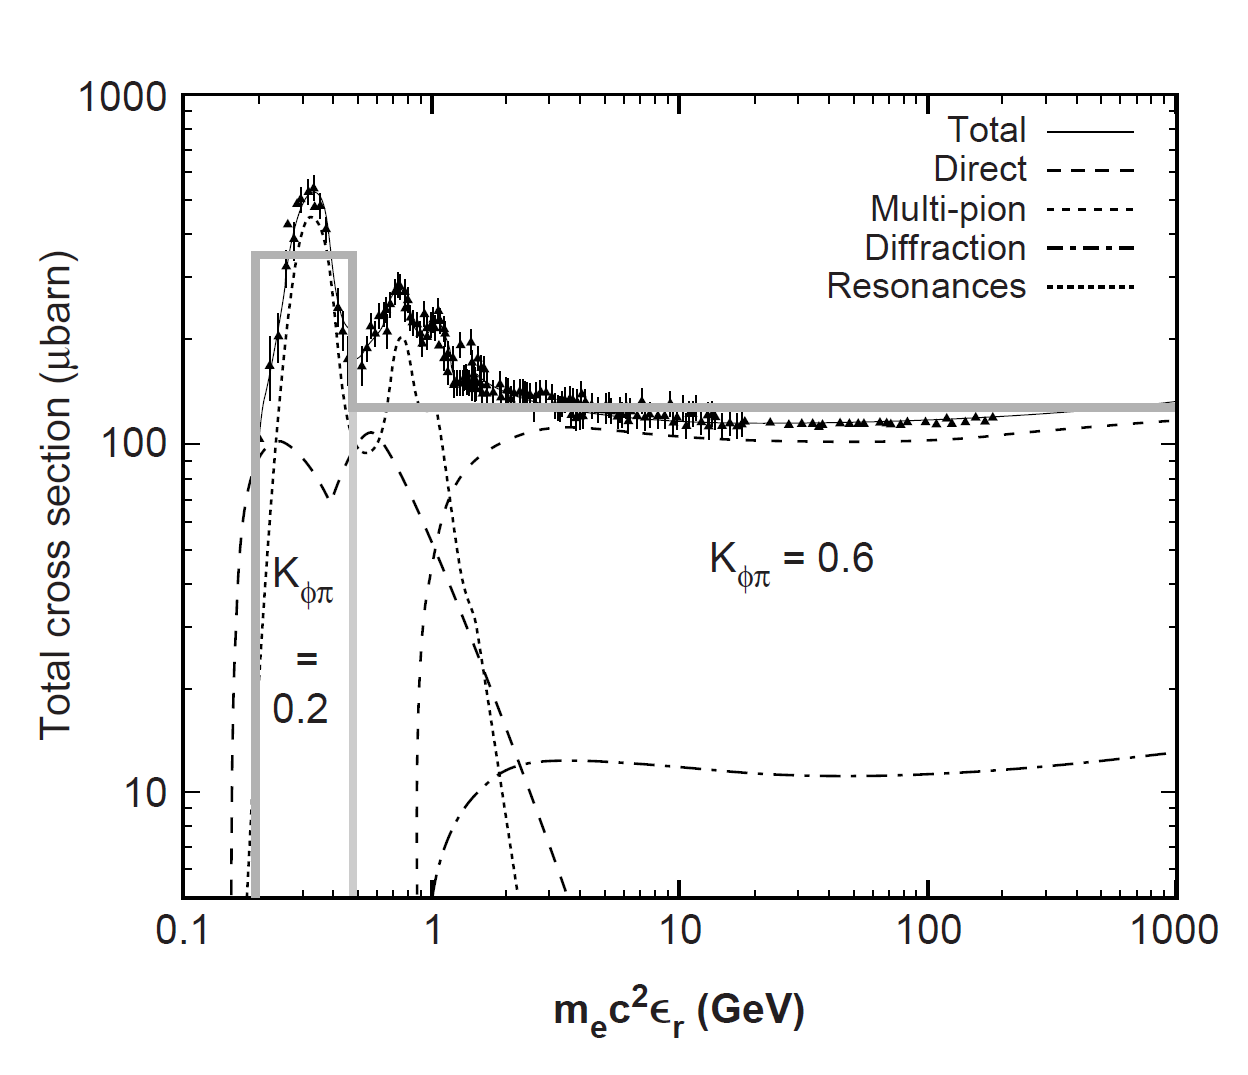
\includegraphics[width=0.5\textwidth]{C:/Users/henri/OneDrive/Documents/NTNU/Semester 10/Masteroppgave/Plots/Dermer_pion_res.png}
    \caption{Pion resonance cross section, and the inelasticity of the interaction. Image taken from \cite{BHradiation}}
    \label{fig:pion_res}
\end{figure}
A Schematic view of the pion resonance cross-section and the inelasticity of the interaction is shown in figure \ref{fig:pion_res}. 

The last important parameter in the pion production timescale is the photon field, and one will be using a photon field as described in section \ref{sec:photon_fields}. The specific photon fields will be determined by what source one is looking at and will be clarified in due time. 

